\documentclass[a4paper,15pt]{article}

%Packages:
\usepackage[utf8]{inputenc}    
\usepackage[vietnamese]{babel} 
\usepackage{graphicx}          
\usepackage{amsmath , amsfonts , amssymb , amsthm} 
\usepackage{hyperref}          
\usepackage{geometry}    
\usepackage{framed}
\usepackage{float}
\usepackage{array}
\usepackage{fancyhdr}
\usepackage{lastpage} % để lấy tổng số trang
\pagestyle{fancy}
\fancyhf{}
\renewcommand{\footrulewidth}{0.4pt}

\fancyfoot[L]{Báo cáo bài tập lớn môn Phương pháp tính nhóm 3 - Học kỳ 242}

% Chân trang bên phải
\fancyfoot[R]{Trang \thepage/\pageref{LastPage}}

\begin{document}
%Trang bìa
\begin{titlepage}
    \centering
    {\textbf{ĐẠI HỌC QUỐC GIA THÀNH PHỐ HỒ CHÍ MINH} \\   
    {\textbf{TRƯỜNG ĐẠI HỌC BÁCH KHOA}} \\   
    {\textbf{BỘ MÔN TOÁN ỨNG DỤNG}} \\
%Chèn logo BK    
\begin{figure}[h]
    \centering
    
\includegraphics[width=0.4\textwidth]{img/logobachkhoa.png}
\end{figure}
%Title
    { \textbf{BÁO CÁO BÀI TẬP LỚN MÔN PHƯƠNG PHÁP TÍNH}} \\
    \hrulefill \\}
    {\huge \textbf{Trình bày phương trình Lotka - Volterra (Mô hình kẻ săn mồi và con mồi) và sử dụng phương pháp Euler để giải hệ phương trình.}} \\
    \vspace{0.5cm}
    
    { \textbf{GVHD: Lê Thị Yến Nhi}} \\
    {\textbf{Nhóm thực hiện: Nhóm 3}}
    \vspace{1cm}

\begin{tabular}{|m{1cm}|m{3cm}|m{3cm}|m{2cm}|}
\hline
STT & Họ và đệm  & Tên &  MSSV \\ \hline
1 & Nguyễn Thái & Hưng & 0000000 \\ \hline
\end{tabular}
\vspace{6cm} \\
\textbf{Thành phố Hồ Chí Minh, tháng 5 năm 2025}
\end{titlepage}

%Muc luc
\tableofcontents
\newpage

%Mo dau
\section{Mở đầu}
\subsection{Lời cảm ơn}
Nhóm em xin gửi lời cảm ơn chân thành nhất đến cô Lê Thị Yến Nhi đã hướng dẫn và hỗ trợ trong quá trình thực hiện bài báo cáo bài tập lớn này. Bài báo cáo đã giúp chúng em hiểu sâu hơn về các khái niệm và nguyên lý liên quan đến đề tài của chúng em nói riêng và môn Phương pháp tính nói chung. Ngoài ra còn giúp chúng em phát triển kỹ năng nghiên cứu và trình bày một bài báo cáo. \\
Chúng em rất trân trọng đến sự quan tâm và hỗ trợ của cô trong quá trình học và thực hiện đề tài này. Mong rằng bài báo cáo lần này của chúng em đã đáp ứng được những kỳ vọng và yêu cầu của cô.
Chúng em xin lắng nghe ý kiến và phản hồi của cô để giúp chúng em hoàn thiện hơn.\\
Lời cuối cùng, chúng em xin cảm ơn cô và chúc cô nhiều sức khỏe và đạt nhiều thành công.
\subsection{Giới thiệu sơ lược về đề tài}
Trong thế giới tự nhiên, mối quan hệ giữa các loài sinh vật – đặc biệt là mối quan hệ giữa kẻ săn mồi và con mồi – là một trong những đề tài thu hút sự quan tâm lớn trong sinh thái học và toán học ứng dụng. Việc mô hình hóa các tương tác này không chỉ giúp chúng ta hiểu rõ hơn về sự biến động quần thể theo thời gian mà còn đóng vai trò quan trọng trong việc dự báo và quản lý tài nguyên sinh học.\\
Một trong những mô hình cổ điển và có ảnh hưởng sâu rộng trong lĩnh vực này là hệ phương trình Lotka–Volterra, thường được dùng để mô tả sự phụ thuộc lẫn nhau giữa hai quần thể: kẻ săn mồi và con mồi. Mô hình này là một hệ phương trình vi phân phi tuyến, cho phép mô tả các chu kỳ tăng giảm quần thể theo cách đơn giản mà vẫn phản ánh được nhiều đặc điểm thực tế.\\
Trong báo cáo này, chúng ta sẽ đi giải quyết 3 vấn đề như sau:
\begin{itemize}
    \item Phương trình Lotka-Volterra (Mô hình kẻ săn mồi và con mồi).
    \item Phương pháp Euler.
    \item Giải phương trình Lotka-Volterra bằng phương pháp Euler.
\end{itemize}
\newpage
%Co so ly thuyet
\section{Cơ sở lý thuyết}
\subsection{Phương trình Lotka-Volterra}
\subsubsection{Nguồn gốc}
Phương trình Lotka–Volterra ra đời đầu thế kỷ 20 nhờ hai nhà khoa học độc lập Alfred J. Lotka (Mỹ) và Vito Volterra (Ý). Ban đầu, Lotka đề xuất mô hình toán học này trong ngữ cảnh phản ứng hoá học tự xúc tác (1910). Sau đó (1920–1925), ông mở rộng nó để mô tả tương tác sinh thái giữa loài thực vật và loài ăn cỏ rồi tiến tới mô hình săn mồi – con mồi. Độc lập, Volterra (1926) cũng phát triển cùng bộ phương trình này để giải thích hiện tượng thú săn (cá săn mồi) tăng đột biến khi điều kiện đánh bắt cá bị giảm trong Chiến tranh thế giới I. Sau khi Volterra biết tới công trình của Lotka, cả hai phương trình được gộp chung và ngày nay gọi là “mô hình Lotka–Volterra”. Mô hình này trở thành nền tảng cho phân tích toán học trong sinh thái học và còn được mở rộng sang nhiều lĩnh vực khác.
\subsubsection{Nội dung}
Mô hình Lotka-Volterra là hai phương trình vi phân phi tuyến bậc nhất, mô tả biến thiên quần thể của con mồi và và kẻ săn mồi, Phương trình có dạng như sau:
\[
    \begin{cases}
    \frac{dx}{dt} = \alpha x - \beta x y \\
    \frac{dy}{dt} = \delta x y - \gamma y
    \end{cases}
\]
Trong đó:
\begin{itemize}
    \item $x(t)$ là số lượng con mồi tại thời điểm $t$.
    \item $y(t)$ là số lượng thú săn tại thời điểm $t$.
    \item $\alpha$ là tốc độ sinh sản tự nhiên của con mồi (khi không có thú săn).
    \item $\gamma$ là tỉ lệ tử vong tự nhiên của thú săn (khi không có con mồi).
    \item $\beta$ là tốc độ săn mồi, mức độ mà thú săn săn được con mồi.
    \item $\delta$ là hiệu suất chuyển hoá, mức độ mà con mồi bị săn chuyển thành sự sinh sản cho thú săn.
\end{itemize}
Ta thấy được:
\begin{itemize}
    \item Phương trình thứ nhất thể hiện con mồi tăng theo hàm mũ (tỉ lệ với số lượng $x$) nhưng bị giảm theo độ săn mồi của kẻ ăn mồi ($\beta x y$).
    \item Phương trình thứ hai biểu diễn thú săn sinh sản tỉ lệ với lượng con mồi tiêu thụ ($\delta x y$) và giảm do tử vong tự nhiên ($\gamma y$).
\end{itemize}
Ví dụ:
\begin{itemize}
    \item Nếu $\beta$ lớn thì mỗi cá thể thú săn tiêu diệt được nhiều con mồi $\rightarrow$ Quần thể con mồi giảm nhanh hơn. 
    \item Nếu $\delta$ lớn thì mỗi con mồi bị ăn sẽ tạo ra nhiều thú săn con $\rightarrow$ Quần thể thú săn tăng nhanh hơn.
\end{itemize}
Để dễ hiểu hơn, ta sẽ phân tích một mô hình thực tế kinh điển của mô hình Lotka-Volterra là mô hình mối quan hệ giữa linh miêu Canada (Lynx canadensis) và thỏ rừng Bắc Mỹ (Lepus americanus) được ghi nhận từ dữ liệu của công ty Hudson's Bay tại Canada trong khoảng 90 năm (1845-1935). Ta có phương trình sau:
\[
\begin{cases}
    \frac{dx}{dt} = \alpha x - \beta x y \\
    \frac{dy}{dt} = \delta x y - \gamma y
\end{cases}
\]
Trong đó:
\begin{itemize}
    \item $x(t)$ là số lượng thỏ rừng Bắc Mỹ (con mồi).
    \item $y(t)$ là số lượng linh miêu Canada (kẻ săn mồi).
    \item $\alpha$ là tốc độ sinh sản tự nhiên của thỏ.
    \item $\beta$ là tỉ lệ thỏ bị linh miêu bắt.
    \item $\gamma$ là tỉ lệ tử vong tự nhiên của linh miêu.
    \item $\delta$ là hiệu suất tăng trưởng của linh miêu nhờ săn thỏ.
\end{itemize}
Chúng ta có thể phân tích như sau:
\begin{itemize}
    \item Thỏ tăng do sinh sản, giảm do bị săn bắt.
    \item Linh miêu tăng do săn được thỏ, giảm do tử vong tự nhiên.
    \item Khi thỏ tăng, linh miêu có thêm nhiều thức ăn $\rightarrow $ Linh miêu tăng theo nhưng sẽ có một khoảng trễ.
    \item Khi linh miêu tăng vượt quá lượng thỏ, cần lượng thức ăn (thỏ) lớn nên lượng thỏ bị ăn nhiều, giảm số lượng $\rightarrow$ Lượng linh miêu cũng giảm theo.
\end{itemize}
\subsubsection{Mục đích và ý nghĩa}
Mục đích chính của mô hình là nghiên cứu động lực quần thể, cụ thể là:
\begin{itemize}
    \item Dự đoán chu kỳ tăng giảm của hai quần thể trong một hệ sinh thái.
    \item Mô phỏng hệ sinh thái đơn giản để hiểu các nguyên lý sinh thái cơ bản.
    \item Phân tích tính ổn định và chu kỳ dao động của hệ sinh vật tương tác với nhau.
    \item Dùng trong sinh thái học, đặc biệt là trong quản lý tài nguyên sinh vật hoặc nghiên cứu mất cân bằng sinh thái.
\end{itemize}
Ý nghĩa trong các lĩnh vực:
\begin{itemize}
    \item Sinh thái học và sinh học
    \begin{itemize}
        \item Mô phỏng tương tác giữa loài (cạnh tranh, cộng sinh, ký sinh, \ldots)
        \item Nghiên cứu hiệu ứng tuyệt chủng và bảo tồn loài
    \end{itemize}
    
    \item Kinh tế học
    \begin{itemize}
        \item Mô hình cạnh tranh giữa hai công ty trên thị trường có thể được biểu diễn giống như con mồi - thú săn.
        \item Mô hình hóa cạnh tranh nguồn lực.
    \end{itemize}
    
    \item Thần kinh học
    \begin{itemize}
        \item Mô tả hoạt động tương tác giữa các nơron ức chế và kích thích.
    \end{itemize}
    
    \item Khoa học dữ liệu và trí tuệ nhân tạo
    \begin{itemize}
        \item Một số mô hình học máy, đặc biệt là trong hệ thống phức tạp, sử dụng nguyên lý tương tự để biểu diễn tương tác giữa các tác nhân (agents).
    \end{itemize}
\end{itemize}
\subsection{Phương pháp Euler}
\subsubsection{Lý thuyết}
Phương pháp Euler là kỹ thuật xấp xỉ sơ cấp nhất để giải bài toán giá trị ban đầu. Mặc dù hiếm khi được sử dụng trong thực tế, sự đơn giản trong phép dẫn giải khiến nó hữu ích để minh họa các kỹ thuật xây dựng một số phương pháp tiên tiến hơn, nhưng không cần đại số phức tạp đi kèm trong các phép xây dựng đó.\\
Mục tiêu của phương pháp Euler là tìm nghiệm xấp xỉ cho bài toán giá trị ban đầu:
\begin{equation}
    \frac{dy}{dt} = f(t, y), \quad a \leq t \leq b, \quad y(a) = \alpha.
\end{equation}
Một nghiệm liên tục \( y(t) \) sẽ không được thu được; thay vào đó, các nghiệm xấp xỉ cho \( y \) sẽ được sinh ra tại các giá trị khác nhau, gọi là các điểm lưới, trong khoảng \( [a, b] \). Khi nghiệm xấp xỉ được tìm tại các điểm này, nghiệm xấp xỉ tại các điểm khác trong khoảng có thể được tìm bằng phép nội suy.

Trước tiên, chúng ta giả định rằng các điểm lưới được phân bố đều trong khoảng \( [a, b] \). Điều kiện này được đảm bảo bằng cách chọn một số nguyên dương \( N \) và xác định các điểm lưới như sau:

\[
t_k = a + k h, \quad \text{với } k = 0, 1, 2, \ldots, N,
\]

Khoảng cách giữa các điểm \( h = \frac{b - a}{N} = t_{k+1} - t_k \) được gọi là bước nhảy (step size).

Chúng ta sẽ sử dụng Định lý Taylor để dẫn ra phương pháp Euler. Giả sử \( y(t) \), nghiệm duy nhất của phương trình (1), có đạo hàm bậc hai liên tục trên \( [a, b] \), sao cho với mỗi \( k = 0, 1, 2, \ldots, N-1 \), ta có:
\[
y(t_{k+1}) = y(t_k) + (t_{k+1} - t_k) y'(t_k) + \frac{(t_{k+1} - t_k)^2}{2} y''(\xi_k),
\]
với một số \( \xi_k \in (t_k, t_{k+1}) \). Vì \( t_{k+1} - t_k = h \), ta có:
\[
y(t_{k+1}) = y(t_k) + h y'(t_k) + \frac{h^2}{2} y''(\xi_k),
\]
Và vì \( y(t) \) thỏa mãn phương trình vi phân (1), nên:
\begin{equation}
    y(t_{k+1}) = y(t_k) + h f(t_k, y(t_k)) + \frac{h^2}{2} y''(\xi_k).
\end{equation}
Phương pháp Euler xây dựng \( w_k \approx y(t_k) \), với mỗi \( k = 1, 2, \ldots, N \), bằng cách bỏ qua số hạng bậc hai. Do đó, phương pháp Euler là:
\[
w_0 = \alpha,
\]
\begin{equation}
    w_{k+1} = w_k + h f(t_k, w_k), \quad \text{với } k = 0, 1, \ldots, N - 1.
\end{equation}
\subsubsection{Công thức Euler}
Cho bài toán:
\[
\frac{dy}{dt} = f(t,y), \quad  y(t_0) = y_0
\]

thì công thức cho phương pháp Euler tính gần đúng các nghiệm tại điểm $t_1,t_2,...,t_n$ là:
\[
\begin{cases}
    x(t_k) \approx x_k = x_{k-1} + h f(t_{k-1}, x_{k-1}, y_{k-1}) \\
    y(t_k) \approx y_k = y_{k-1} + h g(t_{k-1}, x_{k-1}, y_{k-1}) \\
\end{cases}
\quad \text{với } k = 0, 1, 2, \ldots, n
\]
Ngoài ra, ta còn có công thức phương pháp Euler cải tiến như sau:
\[
\begin{cases}
K_{1x} = h f(t_{k-1}, x_{k-1}, y_{k-1}) \\
K_{1y} = h g(t_{k-1}, x_{k-1}, y_{k-1}) \\
K_{2x} = h f(t_{k-1} + h, x_{k-1} + K_{1x}, y_{k-1} + K_{1y}) \\
K_{2y} = h g(t_{k-1} + h, x_{k-1} + K_{1x}, y_{k-1} + K_{1y}) \\
x(t_k) \approx x_k = x_{k-1} + \frac{1}{2}(K_{1x} + K_{2x}) \\
y(t_k) \approx y_k = y_{k-1} + \frac{1}{2}(K_{1y} + K_{2y})
\end{cases}
\]
\subsubsection{Bài toán ví dụ}
Ta sẽ cùng đi giải một bài toán sử dụng phương pháp Euler cải tiến để dễ hình dung hơn. Ta có bài toán như sau:
\[
\begin{cases}
x'(t) = tx - 2y + 1 \\
y'(t) = 2x + ty + \sin t, \quad t \geq 1 \\
x(1) = 0.25 \\
y(1) = 0.75
\end{cases}
\]
Sử dụng công thức Euler cải tiến để xấp xỉ giá trị của $x(t)$ và $y(t)$ tại $t = 1.2$ với bước $h = 0.2$.
\begin{center}
    \textbf{Lời giải}
\end{center}
Ta có: 
\[
t_0 = 1, \quad x_0 = 0.25, \quad y_0 = 0.75,  \quad h = 0.2.
\]
\[
f(t,x,y) = tx - 2y +1;\quad g(t,x,y) = 2x +ty+ \sin t
\]
Với k =1: \\
Đầu tiên, ta tính $K_{1x}$ và $K_{1y}$ tại các điểm $t_0,x_0,y_0$:
\[
\begin{cases}
    K_{1x} = hf(t_0,x_0,y_0) = h(t_0x_0 -2y_0 +1) = 0.2(1 \cdot 0.25 -2\cdot0.75 +1) = -0.05 \\
    K_{1y} = hg(t_0, x_0, y_0) = h(2x_0 + t_0 y_0 + \sin t_0) = 0.2(2 \cdot 0.25 + 1 \cdot 0.75 +\sin 1) =  0.4183
\end{cases}
\]
Tiếp theo, ta tính $K_{2x}$ và $K_{2y}$:
\[
\begin{cases}
K_{2x} = hf(t_0 + h, x_0 + K_{1x}, y_0 + K_{1y}) 
       = h[(t_0 + h)(x_0 + K_{1x}) - 2(y_0 + K_{1y}) + 1] \\
K_{2y} = hg(t_0 + h, x_0 + K_{1x}, y_0 + K_{1y})
       = h[2(x_0 + K_{1x}) + (t_0 + h)(y_0 + K_{1y}) + \sin(t_0 + h)]
\end{cases}
\]
Thu được kết quả như sau:
\[
\begin{cases}
    K_{2x} = 0.2[(1 + 0.2)(0.25 -0.05) -2(0.75 + 0.4183) +1] = -0.2193 \\
    K_{2y} = 0.2[2(0.25 -0.05) + (1 + 0.2)(0.75 + 0.4183) + \sin(1 +0.2)] = 0.5468
\end{cases}
\]
Từ đây, ta có thể tính $x(1.2)  \text{ và } y(1.2) $:
\[
\begin{cases}
    x(1.2) \approx x_1 = x_0 + \frac{1}{2}(K_{1x} + K_{2x}) \\
    y(1.2) \approx y_1 = y_0 + \frac{1}{2}(K_{1y} + K_{2y})
\end{cases}
\]
\[
\rightarrow
\quad 
\begin{cases}
    x(1.2) \approx x_1 = 0.25 + \frac{1}{2}(-0.05 - 0.2193) = 0.1154 \\
    y(1.2) \approx y_1 = 0.75 + \frac{1}{2} (0.4183 + 0.5468) = 1.2326
\end{cases}
\]
Vậy ta đã xấp xỉ giá trị của $x(1.2) \text{ và } y(1.2)$ bằng phương pháp Euler cải tiến.



\section{Ứng dụng phương pháp Euler vào giải phương trình Lotka - Volterra}
\subsection{Công thức Euler trong phương trình Lotka - Volterra}
\subsubsection{Công thức Euler}
Ta có công thức Euler như sau:
\[
    \begin{cases}
    x(t_k) \approx x_k = x_{k-1} + h f(t_{k-1}, x_{k-1}, y_{k-1}) \\
    y(t_k) \approx y_k = y_{k-1} + h g(t_{k-1}, x_{k-1}, y_{k-1}) \\
    \end{cases}
\]
Và phương trình Lotka - Volterra:
\[
    \begin{cases}
    \frac{dx}{dt} = \alpha x - \beta x y \\
    \frac{dy}{dt} = \delta x y - \gamma y
    \end{cases}
\]
Thay công thức Euler vào hệ phương trình trên, ta thu được:
\[
\begin{cases}
x_{k+1} = x_k + h \cdot \left( \alpha x_k - \beta x_k y_k \right) \\
y_{k+1} = y_k + h \cdot \left( \delta x_k y_k - \gamma y_k \right)
\end{cases}
\]
Tuy nhiên, chúng ta thường để điểm bắt đầu là $k=0$ nên ta sẽ chuyển đổi công thức để dễ ứng dụng hơn trong tính toán, ta có phương trình mới như sau:
\[
    \begin{cases}
        x_{k} = x_{k-1} + h \cdot \left( \alpha x_{k-1} - \beta x_{k-1} y_{k-1} \right) \\
y_{k} = y_{k-1} + h \cdot \left( \delta x_{k-1} y_{k-1} - \gamma y_{k-1} \right)
    \end{cases}
\]
\subsubsection{Công thức Euler cải tiến}
Ta có công thức Euler cải tiến như sau:
\[
\begin{cases}
K_{1x} = h f(t_{k-1}, x_{k-1}, y_{k-1}) \\
K_{1y} = h g(t_{k-1}, x_{k-1}, y_{k-1}) \\
K_{2x} = h f(t_{k-1} + h, x_{k-1} + K_{1x}, y_{k-1} + K_{1y}) \\
K_{2y} = h g(t_{k-1} + h, x_{k-1} + K_{1x}, y_{k-1} + K_{1y}) \\
x(t_k) \approx x_k = x_{k-1} + \frac{1}{2}(K_{1x} + K_{2x}) \\
y(t_k) \approx y_k = y_{k-1} + \frac{1}{2}(K_{1y} + K_{2y})
\end{cases}
\]
Và phương trình Lotka - Volterra:
\[
    \begin{cases}
    \frac{dx}{dt} = \alpha x - \beta x y \\
    \frac{dy}{dt} = \delta x y - \gamma y
    \end{cases}
\]
Thay công thức Euler cải tiến vào hệ phương trình, ta thu được:
\[
\begin{cases}
K_1^x = h \cdot \left( \alpha x_k - \beta x_k y_k \right) \\
K_1^y = h \cdot \left( \delta x_k y_k - \gamma y_k \right) \\
K_2^x = h \cdot \left[ \alpha (x_k + K_1^x) - \beta (x_k + K_1^x)(y_k + K_1^y) \right] \\
K_2^y = h \cdot \left[ \delta (x_K + K_1^x)(y_k + K_1^y) - \gamma (y_k + K_1^y) \right] \\
x_{k+1} = x_k + \frac{1}{2} \left( K_1^x + K_2^x \right) \\
y_{k+1} = y_k + \frac{1}{2} \left( K_1^y + K_2^y \right)
\end{cases}
\]
\subsection{Tính toán thủ công}
Giả sử quần thể của thỏ và sói được mô tả bằng phương trình Lotka – Volterra với các hệ số $\alpha = 0.08; \beta = 0.001; \delta = 0.00008; \gamma = 0.02.$ Thời gian t được tính theo tháng. Vào thời điểm ban đầu biết lượng thỏ là 1000, lượng sói là 40. Hãy ước tính số lượng thỏ và sói trong 12 tháng tới.
\begin{center}
    \textbf{Lời giải}
\end{center}
Ta nhận thấy thỏ là con mồi và sói là động vật săn mồi. Nên ta có hệ phương trình sau:
\[
\begin{cases}
    \frac{dx}{dt} = 0.08 x - 0.001 x y \\
    \frac{dy}{dt} = 0.00008 x y - 0.02 y
\end{cases}
\]
Do thời gian t được tính bằng tháng, ta chọn bước nhảy h = 1 tháng. Từ đó được hệ:
\[
\begin{cases}
    x(t_{k+1}) = x(t_k) + x'(t_k) \\
    y(t_{k+1}) = y(t_k) + y'(t_k)
\end{cases}
\]
Đầu tiên, ta sẽ xét tại $t= t_1$:
\[
\begin{cases}
    x(t_1) = x_0 + h(\alpha  x_0 - \beta  x_0 y_0) \\
y(t_1) = y_0 + h(\delta x_0y_0 - \gamma y_0) 
\end{cases}
\]
Từ đó ta có kết quả tại $t= t_1$:
\[
\begin{cases}
    x(t_1) = 1000 + (0.08   \cdot 1000 - 0.001 \cdot 1000 \cdot 40) = 1040\\
    y(t_1) = 40 + ( 0.00008\cdot 1000 \cdot 40 - 0.02 \cdot 40) = 42.4
\end{cases}
\]
Tiếp tục thực hiện tính toán, ta thu được bảng sau:
\begin{table}[H]
\centering
\begin{tabular}{|c|c|c|}
\hline
\textbf{Tháng} & \textbf{Số lượng thỏ} & \textbf{Số lượng sói} \\
\hline
0  & 1000 & 40 \\
1  & 1040 & 42 \\
2  & 1079 & 45 \\
3  & 1117 & 48 \\
4  & 1152 & 51 \\
5  & 1185 & 55 \\
6  & 1215 & 59 \\
7  & 1240 & 64 \\
8  & 1260 & 69 \\
9  & 1274 & 74 \\
10 & 1281 & 81 \\
11 & 1281 & 87 \\
12 & 1271 & 94 \\
\hline
\end{tabular}
\caption{Số lượng thỏ và sói từ tháng đầu tiên đến tháng 12.}
\end{table}
Vậy sau 12 tháng thì


\begin{itemize}
    \item Số lượng thỏ là 1271.
    \item Số lượng sói là 94.
\end{itemize}
Như vậy, dựa vào phương pháp Euler, ta đã giải được phương trình Lotka – 
Volterra và ước lượng số lượng thỏ và sói tương ứng trong 12 tháng. Nhìn vào bảng ta thấy vào những tháng đầu tiên, số lượng thỏ tăng rất nhanh dẫn đến số lượng sói tăng nhanh theo. Nhưng khi tính tới những tháng cuối, số lượng sói tuy vẫn tăng rất nhanh, thậm chí là còn nhanh hơn lúc đầu, trái lại số lượng thỏ lại tăng chậm dần sau đó dừng tăng ở tháng thứ 11 và bắt đầu giảm từ tháng thứ 12. Điều này có thể hiểu là do lượng thỏ tăng ở những tháng đầu đã cung cấp nguồn thức ăn dồi dào cho cho sói, làm lượng sói tăng nhanh theo. Nhưng càng ngày lượng sói càng tăng, càng săn nhiều thỏ hơn do đó làm lượng thỏ tăng chậm lại, cho đến khi lượng sói trở nên quá nhiều. Lúc này thỏ không sinh sản kịp để bù lại lượng bị sói săn dẫn đến số lượng thỏ bị sụt giảm. Trong 
tương lai khi lượng thỏ giảm đến mức cực tiểu thì sẽ lại làm lượng sói tăng chậm rồi giảm, từ đó lượng thỏ lại tăng lên. Qua đó có thể nói, phương trình Lotka – Volterra đã phần nào khái quát rõ nét chu kỳ của hệ sinh thái khi xảy ra sự chênh lệch lớn giữa 2 loài.
\subsection{Giải bài tập bằng MATLAB}
\subsubsection{Code}
Việc tính toán thủ công các bài toán liên quan đến phương trình Lotka - Volterra bằng việc sử dụng phương pháp Euler tuy đơn giản nhưng lại rất tốn thời gian để giải ra. Nên chúng ta sẽ sử dụng đến phần mềm MATLAB để lập trình tính toán nhanh chóng hơn.\\
\newpage
Ta có đoạn code để tìm số lượng của 2 loài sau khoảng thời gian $t$ như dưới đây:
\begin{verbatim}
% Nhập giá trị tmax và bước nhảy h 
    t0 = 0;
    disp('tmax là thời gian muốn khảo sát'); 
    tmax = input('Nhập giá trị tmax= '); 
    h = input('Nhập giá trị bước nhảy h='); 
% Tính số bước nhảy 
    n = floor((tmax - t0) / h); 
% Khởi tạo mảng x và y 
    x = zeros(1, n + 1); 
    y = zeros(1, n + 1); 
% Nhập giá trị ban đầu của x và y 
    disp('x0 là số lượng con mồi ban đầu'); 
    disp('y0 là số lượng kẻ săn ban đầu'); 
    x(1) = input('Nhập giá trị của x tại thời điểm ban đầu là x0= '); 
    y(1) = input('Nhập giá trị của y tại thời điểm ban đầu là y0= '); 
% Nhập các hệ số 
    disp('Hãy nhập các hệ số ảnh hưởng đến x, y (A, B, C, D > 0)'); 
    a = input('Nhập hệ số tăng trưởng của con mồi: A= '); 
    c = input('Nhập hệ số suy giảm của kẻ săn: C= '); 
    b = input('Nhập hệ số suy giảm của con mồi do kẻ săn: B= '); 
    d = input('Nhập hệ số xác định độ tăng trưởng của kẻ săn khi mất một con mồi: D= '); 
    fprintf('Ta có hệ:\n'); 
    fprintf('x''(t) = %.2f x(t) - %.2f x(t) y(t)\n', a, b); 
    fprintf('y''(t) = %.2f x(t) y(t) -%.2f y(t)\n', c, d); 
% Giải hệ phương trình sử dụng phương pháp Euler 
    for i = 1:n 
    t = t0 + i * h; 
    x(i + 1) = x(i) +  (a * x(i) - b * x(i) * y(i)); 
    y(i + 1) = y(i) +  (d * x(i) * y(i) -c * y(i)); 
    end 
    fprintf('Giá trị x(%f) và y(%f) lần lượt là\n', t, t); 
    fprintf('x = %f, y = %f\n', x(end), y(end)); 
% Vẽ đồ thị kết quả 
    time = t0:h:tmax; 
    figure; 
    plot(time, x, 'b', 'DisplayName', 'x (Con mồi)'); 
    hold on; 
    plot(time, y, 'r', 'DisplayName', 'y (Kẻ săn)'); 
    xlabel('Thời gian'); 
    ylabel('Số lượng'); 
    legend(); 
    title('Mô hình Lotka-Volterra'); 
    grid on; 
    hold off;
\end{verbatim}
\newpage
\subsubsection{Ứng dụng code giải bài toán}
Đầu tiên, ta sẽ quay trở lại giải bài toán đã tính thủ công để kiểm tra kết quả.


\textbf{Câu 1: }Giả sử quần thể của thỏ và sói được mô tả bằng phương trình Lotka – Volterra với các hệ số $\alpha = 0.08; \beta = 0.001; \delta = 0.00008; \gamma = 0.02.$ Thời gian t được tính theo tháng. Vào thời điểm ban đầu biết lượng thỏ là 1000, lượng sói là 40. Hãy ước tính số lượng thỏ và sói trong 12 tháng tới.
\begin{center}
    \textbf{Lời giải}
\end{center}
Đầu tiên, ta đi phân tích các dữ liệu:
\begin{itemize}
    \item Thời gian (tmax) = 12 tháng
    \item Bước nhảy (h) = 1
    \item Số lượng thỏ ban đầu (x0) = 1000
    \item Số lượng sói ban đầu (y0) = 40 
    \item Tốc độ sinh sản tự nhiên của thỏ (a) = 0.08
    \item Tốc độ chết tự nhiên của sói (c) = 0.02
    \item Tốc độ suy giảm của thỏ do sói (b) = 0.001
    \item Tốc độ sinh sản của sói từ việc săn mồi (d) = 0.00008
\end{itemize}
Ta nhập các giá trị trên vào code như sau:\\
\begin{figure}[H]
    \centering
    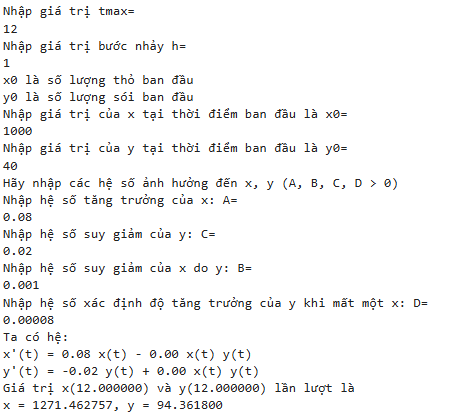
\includegraphics[scale=0.75]{img/Nhapvao.png}
    \caption{Nhập thông số.}
    \label{fig:enter-label}
\end{figure}
Ta thu được đồ thị như dưới đây: \\
\begin{figure}[H]
    \centering
    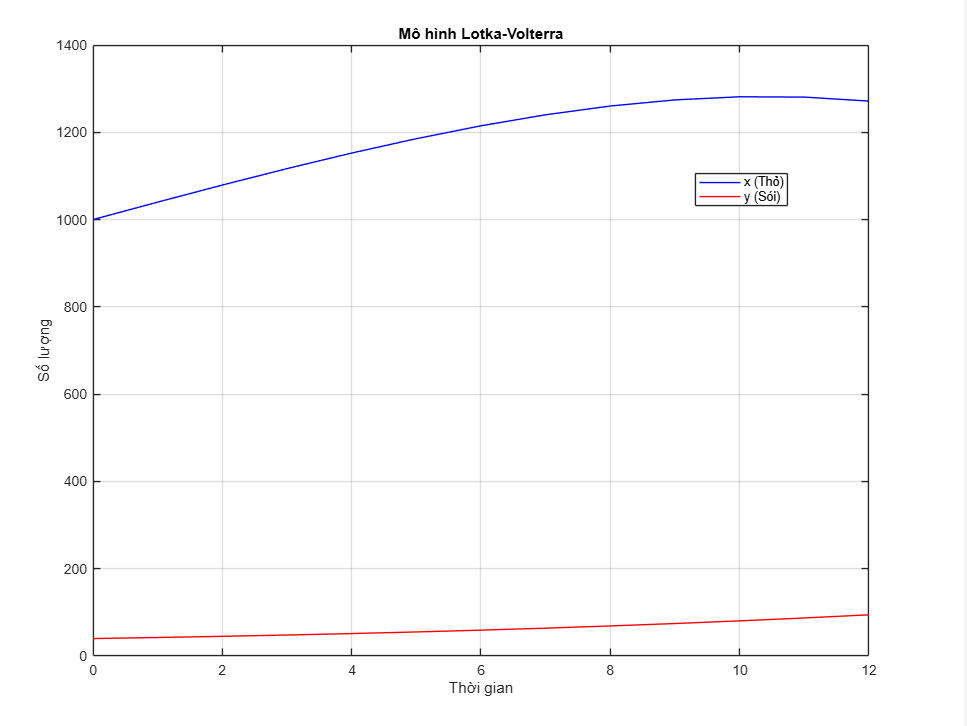
\includegraphics[scale=0.5]{img/Dothibai1.png}
    \caption{Đồ thị thu được từ bài 1.}
    \label{fig:enter-label}
\end{figure} 
\textbf{Câu 2:} 
Giả sử các quần thể hươu và báo được mô tả bằng phương trình Lotka-Volterra với các hệ số a =0.06 , b= 0.0006, c = 0.03 , d= 0.00009 và thời gian t được tính theo tháng. Biết vào thời điểm ban đầu số lượng hươu là 800 con, số lượng báo là 35 con. Hãy ước tính số lượng hươu và báo trong 30 tháng tới bằng phương pháp Euler.
\begin{center}
    \textbf{Lời giải}
\end{center}
Ta xác định được:
\begin{itemize}
    \item Hươu là con mồi.
    \item Báo là kẻ săn mồi.
\end{itemize}
Ta sẽ nhập vào code như sau:
\begin{figure}[H]
    \centering
    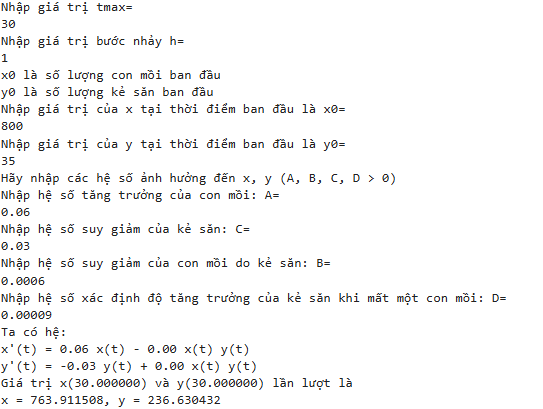
\includegraphics[scale=0.75]{img/Nhapvao2.png}
    \caption{Nhập thông số bài 2.}
    \label{fig:enter-label}
\end{figure}
Ta thu được đồ thị như sau:
\begin{figure}[H]
    \centering
    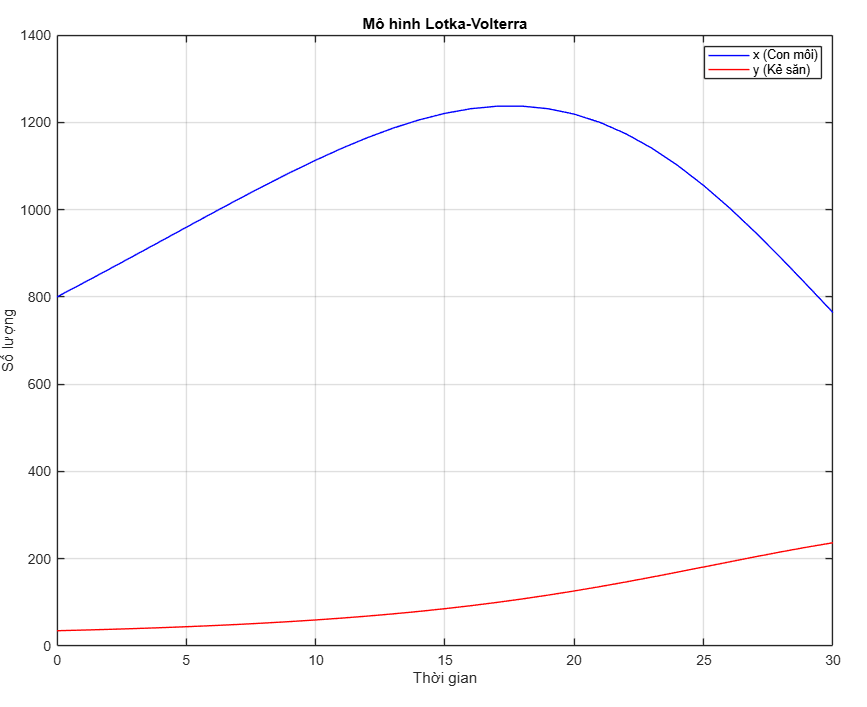
\includegraphics[scale=0.5]{img/Dothibai2.png}
    \caption{Đồ thị thu được từ bài 2.}
    \label{fig:enter-label}
\end{figure}
\section{Tài liệu tham khảo}
\begin{thebibliography}{9}
\bibitem{Burden}
Richard L. Burden and J. Douglas Faires,
\textit{Numerical Analysis (9th ed.)}
\bibitem{LeThaiThanh}
Lê Thái Thanh,
\textit{Giáo trình Phương pháp tính},
 NXB: ĐHQG-HCM 
\bibitem{LTYN}
Lê, Thị Yến Nhi.
\textit{"Bài giảng Phương pháp tính - Chương 4: Phương trình vi phân"}, 2025, Trường Đại học Bách khoa, ĐHQG-HCM. Slide Powerpoint.
\end{thebibliography}
\end{document}